\documentclass[english, DIV=13]{scrartcl}

\usepackage[utf8x]{inputenc}
\usepackage[T1]{fontenc}
\usepackage{lmodern}
\usepackage{microtype}
\usepackage{xspace}
\usepackage[binary-units=true]{siunitx}
\usepackage{graphicx}
\usepackage{hyperref}
\usepackage{todonotes}
\usepackage{epstopdf}
\usepackage{array}
\usepackage{multicol}
\usepackage{multirow}
\usepackage{tabularx} % tabular with automatic line-break
\newcolumntype{Y}{>{\centering\arraybackslash}X} % centered column
\usepackage{amsmath}
\usepackage{grffile} % better name handling with graphicx
\usepackage{currfile} % provides relative file inclusion for tikzscale
\usepackage{listings}
\lstset{%
    basicstyle=\scriptsize\ttffamily,
    breaklines=true
}

\usepackage{tikz}
\usepackage{pgfplots}
\usepackage{pgfplots}
\usepackage{tikzscale}
\pgfplotsset{compat=newest}
\usetikzlibrary{plotmarks}
\usepackage{rotating}
\usepackage[absolute,overlay]{textpos}
\usepackage{circuitikz}

% Math symbols
\usepackage{amsmath}
\usepackage{amssymb}
\usepackage{amsthm}
\DeclareMathOperator*{\argmin}{arg\,min}
\DeclareMathOperator*{\argmax}{arg\,max}
\newcommand\norm[1]{\left\lVert#1\right\rVert}

% Sets
\newcommand{\Z}{\mathbb{Z}}
\newcommand{\R}{\mathbb{R}}
\newcommand{\Rn}{\R^n}
\newcommand{\Rnn}{\R^{n \times n}}
\newcommand{\C}{\mathbb{C}}
\newcommand{\K}{\mathbb{K}}
\newcommand{\Kn}{\K^n}
\newcommand{\Knn}{\K^{n \times n}}

% Unit vectors
\usepackage{esint}
\usepackage{esvect}
\newcommand{\kmath}{k}
\newcommand{\xunit}{\hat{\imath}}
\newcommand{\yunit}{\hat{\jmath}}
\newcommand{\zunit}{\hat{\kmath}}
\newcommand{\uunit}{\hat{\umath}}

% rot & div & grad & lap
\DeclareMathOperator{\newdiv}{div}
\newcommand{\divn}[1]{\nabla \cdot #1}
\newcommand{\rotn}[1]{\nabla \times #1}
\newcommand{\grad}[1]{\nabla #1}
\newcommand{\gradn}[1]{\nabla #1}
\newcommand{\lap}[1]{\nabla^2 #1}

% Elec
\newcommand{\B}{\vec B}
\newcommand{\E}{\vec E}
\newcommand{\EMF}{\mathcal{E}}
\newcommand{\perm}{\varepsilon} % permittivity

\newcommand{\bigoh}{\mathcal{O}}
\newcommand\eqdef{\triangleq}

\DeclareMathOperator{\newdiff}{d} % use \dif instead
\newcommand{\dif}{\newdiff\!}
\newcommand{\fpart}[2]{\frac{\partial #1}{\partial #2}}
\newcommand{\ffpart}[2]{\frac{\partial^2 #1}{\partial #2^2}}
\newcommand{\fdpart}[3]{\frac{\partial^2 #1}{\partial #2\partial #3}}
\newcommand{\fdif}[2]{\frac{\dif #1}{\dif #2}}
\newcommand{\ffdif}[2]{\frac{\dif^2 #1}{\dif #2^2}}
\newcommand{\constant}{\ensuremath{\mathrm{cst}}}


\title{LELEC2103}
\subtitle{Project in Electricity 3 : Electronic systems}
\author{Gaëtan Cassiers\and Antoine Paris}
\date{\today}

\begin{document}
\maketitle

\section*{Introduction}
The objective of this project in electronic systems is to design and implement a
two-player video game using a Raspberry-Pi 3, a DE0-Nano board containing an FPGA
and a collection of interfaces and peripherals, and a multi-touch LCD module on
each side. In addition, the FPGA features a Nios II processor running µC/OS-II, a
real-time kernel.
One of the main specificity of this project is that each side is designed and
implemented by two independent groups. However, because the two players have to
communicate with
each other throught a Wi-Fi communication between the two Raspberry-Pis, a common
network interface has been specified by the two groups. This is discussed
in section~\ref{sec:net-interface}. Before that, section~\ref{sec:gameplay-features}
introduces the game that inspired our game and the additional features we decided to
add to it. Section~\ref{sec:global-view} then describes the global architecture of
our game as a block diagram where each block, named subsystem in what follows, serves a
particular purpose. One of the key feature of our implementation of the game is the
3D rendering. Together with the frame compression system we designed, this really
constitutes the core of our project. These two subsystems are discussed in sections
\ref{sec:rendering} and~\ref{sec:compression} respectively.
To ensure robust and fast communication between the Raspberry-Pi and the FPGA, a smart
SPI slave subsystem together with a simple, yet reliable, communication protocol has
been designed and implemented. This is the topic of section~\ref{sec:spi}. Next, in
section~\ref{sec:display-mngt}, the hardware behind the double buffering technique
-- used to avoid tearing effects on the screen -- is explained.
In section~\ref{sec:input-det}, we head to the tasks running on the real-time kernel.
These tasks are responsible for the sensing of the touchscreen and the accelerometer.
Another originality of our game is that the players have the possibility to take a
selfie, either with a smartphone or a PC, to actually see themselves in the game.
Section~\ref{sec:pic-acq} explains this player pictures acquisition subsystem.

\section{Gameplay and features}
\label{sec:gameplay-features}

\subsection{Original game}
Our game is inspired by an existing game available on most smartphones and tablets
and developped by Ketchapp. Figure~\ref{fig:original-game} is a screenshot from this game.
In this original version of the game, the player (represented by the yellow cube on figure
~\ref{fig:original-game}) has to place itself correctly on the white structure in order
to fit in the hole of the wall coming in his direction at a constant speed. The objective
is to pass in as much wall as possible. Passing a wall gives 1 point, failing to pass a
wall makes the score starting back at 0.

\begin{figure}
    \centering
    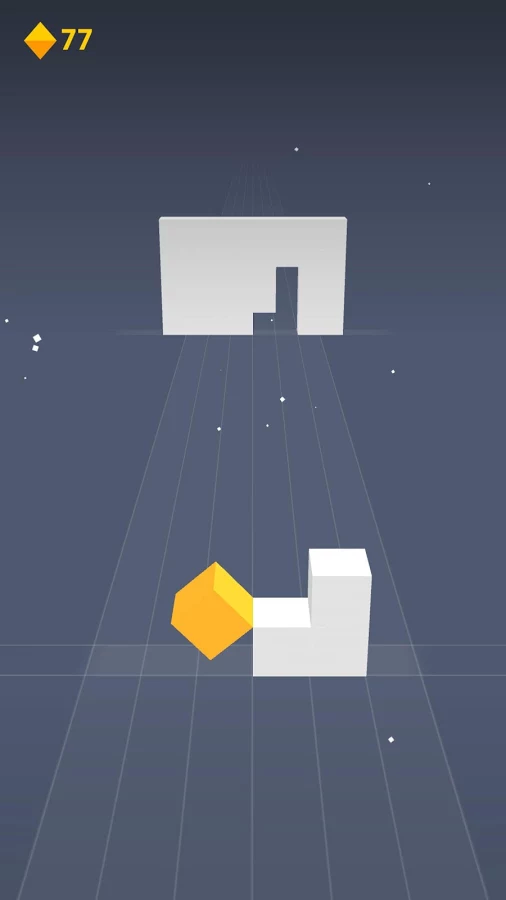
\includegraphics[width=0.3\textwidth]{img/original-game}
    \caption{Screenshot of the orginal game by Ketchapp.}
    \label{fig:original-game}
\end{figure}

\subsection{Custom version of the game}
Our version of the game differs from the original one in several aspects. First, this
is a two-players collaborative game. Second, a game only lasts a finite amount of time
and the two players can control the speed of the wall using the accelerometer.
Finally, failing to pass a wall only decreases the current score by 1. 

\begin{figure}
    \centering
    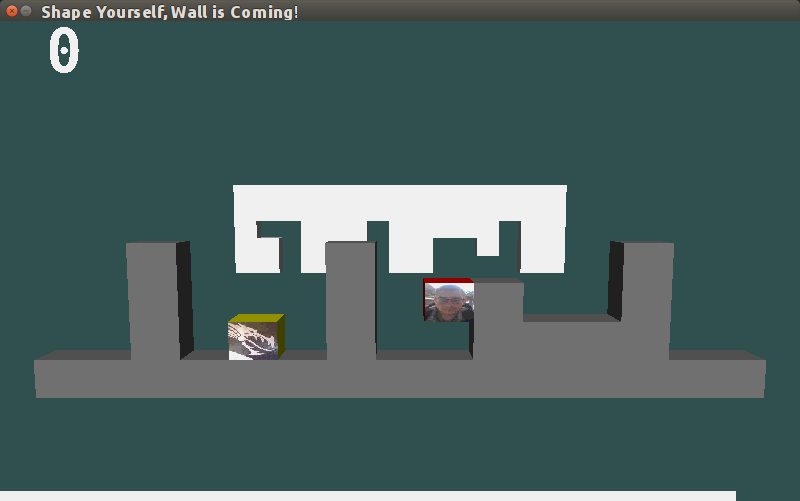
\includegraphics[width=0.7\textwidth]{img/custom-game-version}
    \caption{Screenshot of our version of the game. This screenshot has been taken
    on the PC version of the game but there is really no difference with the actual
    on-device version.}
    \label{fig:custom-game}
\end{figure}

\subsection{Additional features}
The difficulty of the game relies mainly on the fact that the scene is represented as a
3D image. Experience has shown that this can sometimes be really perturbating or even
induces the players in error. To counteract a bit this, and to add some fun to the
gameplay, the player can change de point of view of the 3D scene by tilting the tablet
on the left or on the right. In addition, the player has the possibility to make the
structure on which it stands disappear during a very small amount of time each round.
This feature can also help the player to better see where he should go to fit in the hole.

As briefly mentioned in the introduction, players also have the possibility to take a
selfie, either with a smartphone or a PC, to actually see themselves in the game. More
precisely, their picture appears on the cube they incarnate. In addition to beeing just a
cool feature, this helps the players to localize the cube they control at the start of
each round.

Finally, since playing our game requires a lot of concentration, players can pause the
game whenever they want to take a break.

\section{Network interface}
\label{sec:net-interface}
The way the two players communicate with each other is illustrated in figure~\ref{fig:
comm-scheme}. The approach taken here is client-server based. The server is responsible
for all the logic of the game and maintains an object representing the state of the game.
Centralizing computations in this way ensures a complete synchronization between clients.

A complete communication protocol was rigorously defined by the two groups. This
protocol defines an handshake procedure between a client and the server to ensure both
sides are ready before starting. Once the game has started, the two clients can send
messages to the server based on user inputs (accelerometer values, touch, or gesture).
The server then performs some computations on the game state such as computing player
positions, speed of the wall, remaining time, score, etc. Finally, the server
broadcasts the parts of the game state which changed.

On the practical side, one Raspberry-Pi runs both the server and a client while the other
one only runs a client.

\begin{figure}
    \centering
    \includegraphics[width=1.0\textwidth]{img/global_comm_scheme_cropped.pdf}
    \caption{Block diagram of the network communication.}
    \label{fig:comm-scheme}
\end{figure}

\section{Global view of the client system}
\label{sec:global-view}

The global view of the client system is represented in figure~\ref{fig:global-desktop}
and figure~\ref{fig:global-device}. Through the network interface described in the
previous section, the client builds its own image of the game state. This client game
state is then fed to the rendering subsystem which produces a 3D image. This image
is then compressed and sent to the hardware interface.

One of the strength of our system is this hardware interface. This abstraction offers
a common layer to communicate both with a PC or a device.
On PC, touches, gestures and accelerometer values are simulated with the keyboard.
This eased a lot the development process by allowing efficient debugging first on PC,
and then only on device if necessary.

On PC, the hardware interface mainly interacts with a Python library dedicated to game
developement named Pygame. As a first development step, Pygame allowed us to develop
a fully functionnal basic 2D version of the game. The move to the 3D version
complicated a lot the rendering subsystem. This is explained in
section~\ref{sec:rendering}.

\begin{figure}
    \centering
    \includegraphics[width=0.6\textwidth]{img/block_global_desktop_cropped.pdf}
    \caption{Block diagram of the client, when running on a PC.}
    \label{fig:global-desktop}
\end{figure}

On device, the hardware interface communicates through SPI with the FPGA.
Different types of informations flow in both directions. From the Raspberry-Pi to the
FPGA, compressed frames representing 3D scenes along with control signals for the
display manager are sent at a fixed rate. The reasons why we need a compression
subsystem between the rendering subsystem and the hardware interface are detailed in
section~\ref{sec:compression}. From the Nios processor running µC/OS-II, accelerometer
values and touchscreen events are periodically read out by the hardware interface.


\begin{figure}
    \centering
    \includegraphics[width=0.6\textwidth]{img/block_global_device_cropped.pdf}
    \caption{Block diagram of the client, when running the raspberry-pi/DE0-Nano system.}
    \label{fig:global-device}
\end{figure}

\section{Rendering subsystem}
\label{sec:rendering}

\begin{figure}
    \centering
    \includegraphics[width=0.6\textwidth]{img/block_rendering_cropped.pdf}
    \caption{Pipeline for the rendering of the video.}
\end{figure}

\section{Compression subsystem}
\label{sec:compression}

\subsection{Objectives}

The need for a compression system comes from the following observation:
when transferring 25 frames of 800x480 pixels per second, with 12 bits per pixel,
the bandwidth needed is \SI{115}{Mb/s}. The memory needed for each frame
is \SI{600}{kB}.

In our system, the SPI bandwidth available to transfer the video is \SI{5}{Mb/s},
and the memory available on the FPGA (considering onchip memory only, the SDRAM
being used by the Nios/µC0S-II system) is \SI{30}{kB} per frame.

We thus need a compression by a factor larger than 20, that is such that
the video can be compressed in real-time. The decompression must be done
pixel per pixel, on-the-fly, since there is no memory available to store the
decompressed images.

\subsection{Principle}

\begin{figure}
    \centering
    \includegraphics[width=0.65\textwidth]{img/compression_scheme_cropped.pdf}
    \caption{Principle view of the compression scheme.}
    \label{fig:compression}
\end{figure}

The compression system is based on three steps (see fig.~\ref{fig:compression}):
the color quantization, the run-length coding, and the Huffman coding. The first
step is lossy, while the two other steps are lossless.

\paragraph{Color quantization} The precision for each color channel is
reduced to 4 bits. This step is a preprocessing step that makes it possible
to implement and improves the efficiency of the following steps.

\paragraph{Run-length coding} The image, represented as a list of pixels,
is converted to a list of pairs $(\text{color}, \text{number of repetitions})$.
The allowed sizes for the number of repetitions are
$1, 2, 3, ..., 16,$ $32, 64, ..., 4096$. This allows to encode most images with
a number of blocks that is not too far from the optimum, while keeping the set
of number of repetitions small, which is required for the Huffman compression.

\paragraph{Huffman coding} Two Huffman trees are built: one for the pixels colors
and one for the numbers of repetitions. Each element of the pairs generated
at the previous stage is encoded with the corresponding Huffman tree.
All the codewords are then concatenated together to form the compressed image.

\subsection{Impact of the color quantization}

The color quantization serves different purposes. For the run-length coding,
the quantization creates chunks of constant color when there is a
continuous shading. For the Huffman
coding, the reduction of the pixels length from \SI{24}{bits} to
\SI{12}{bits} means the size of the colorspace is reduced from
\SI{16}{M} to \SI{4}{K}. This simplifies a lot the Huffman coding:
\begin{itemize}
    \item it is much easier to estimate the distribution of the colors
    to build the Huffman tree\footnote{The color and run-length distribution are
    estimated from a set of training images at compile time.};
    \item it keeps the codewords length small, which simplifies the implementation:
    the memory bandwidth required is smaller;
    \item it reduces the amount of logic gates required to implement a decoder,
    which makes it possible to fit it on the FPGA;
    \item it also makes the software encoder faster, for the same reasons
    (memory bandwidth, code size).
\end{itemize}

The color quantization has an impact on the quality of the images
but it is mainly visible on image area exhibiting a color gradient.
For these kinds of images,
it may introduce a "staircase" effect. To avoid this artefact to be visible,
the rendering process has been tuned to avoid producing color gradients
through the choice of an appropriate lightning scheme for the 3D scene (the lightning
has only the directionnal component of the phong lightning model).

\section{SPI slave subsystem}
\label{sec:spi}

\begin{figure}
    \centering
    \includegraphics[width=0.5\textwidth]{img/spi_state_machine_cropped.pdf}
    \caption{State machine for the SPI communication protocol.}
\end{figure}

\section{Display management}
\label{sec:display-mngt}

The system uses double buffering to avoid tearing in displayed images.
It is implemented by two RAMs on the FPGA (see fig.~\ref{fig:display-manager}).

The RAMs are connected to the decoder
(which decodes the code discussed in section~\ref{chap:compression})
through a MUX controlled by a \texttt{display control} register.

The RAMs are also connected to the SPI MMU. The write enable
signal of the RAMs are masked by the \texttt{display control} signal,
so that only RAM that is not connected to the decoder is written.

The \texttt{display control} register can be read from the SPI MMU,
and can be written by the SPI MMU, but only through a buffer register,
in order for changes of \texttt{display control} to be synchronized
to the \texttt{end of frame} signal from the display controller.
This synchronization system avoids tearing.

\begin{figure}
    \centering
    \includegraphics[width=\textwidth]{img/display_manager_cropped.pdf}
    \caption{Block diagram of the display management and synchronization system.}
    \label{fig:display-manager}
\end{figure}

\section{Input detection subsystem}
\label{sec:input-det}

\begin{figure}
    \centering
    \includegraphics[width=0.5\textwidth]{img/tasks_mC_cropped.pdf}
    \caption{Tasks and their relationships on the uC/OS-II operating system.}
\end{figure}

\section{Player pictures acquisition}
\label{sec:pic-acq}

\begin{figure}
    \centering
    \includegraphics[width=0.5\textwidth]{img/block_pictures_cropped.pdf}
    \caption{Block diagram of the picture acquisition subsystem.}
\end{figure}

\section{Conclusion}

\end{document}
